% NB: use pdflatex to compile NOT pdftex.  Also make sure youngtab is
% there...

% converting eps graphics to pdf with ps2pdf generates way too much
% whitespace in the resulting pdf, so crop with pdfcrop
% cf. http://www.cora.nwra.com/~stockwel/rgspages/pdftips/pdftips.shtml




\documentclass[10pt,aspectratio=169,dvipsnames]{beamer}
\usetheme[color/block=transparent]{metropolis}

\usepackage[absolute,overlay]{textpos}
\usepackage{booktabs}
\usepackage[utf8]{inputenc}


\usepackage[scale=2]{ccicons}

\usepackage[official]{eurosym}

%use this to add space between rows
\newcommand{\ra}[1]{\renewcommand{\arraystretch}{#1}}


\setbeamerfont{alerted text}{series=\bfseries}
\setbeamercolor{alerted text}{fg=Mahogany}
\setbeamercolor{background canvas}{bg=white}


\newcommand{\R}{\mathbb{R}}

\def\l{\lambda}
\def\m{\mu}
\def\d{\partial}
\def\cL{\mathcal{L}}
\def\co2{CO${}_2$}



% for sources http://tex.stackexchange.com/questions/48473/best-way-to-give-sources-of-images-used-in-a-beamer-presentation

\setbeamercolor{framesource}{fg=gray}
\setbeamerfont{framesource}{size=\tiny}


\newcommand{\source}[1]{\begin{textblock*}{5cm}(10.5cm,8.35cm)
    \begin{beamercolorbox}[ht=0.5cm,right]{framesource}
        \usebeamerfont{framesource}\usebeamercolor[fg]{framesource} Source: {#1}
    \end{beamercolorbox}
\end{textblock*}}

\usepackage{hyperref}


\usepackage{tikz}
\usetikzlibrary{arrows.meta}

\usepackage[europeanresistors,americaninductors]{circuitikz}


%\usepackage[pdftex]{graphicx}


\graphicspath{{graphics/}}

\DeclareGraphicsExtensions{.pdf,.jpeg,.png,.jpg}



\def\goat#1{{\scriptsize\color{green}{[#1]}}}



\let\olditem\item
\renewcommand{\item}{%
\olditem\vspace{5pt}}

\title{Energy System Modelling\\ Summer Semester 2020, Lecture 3}
%\subtitle{---}
\author{
  {\bf Dr. Tom Brown}, \href{mailto:tom.brown@kit.edu}{tom.brown@kit.edu}, \url{https://nworbmot.org/}\\
  \emph{Karlsruhe Institute of Technology (KIT), Institute for Automation and Applied Informatics (IAI)}
}

\date{}


\titlegraphic{
  \vspace{0cm}
  \hspace{10cm}
    \includegraphics[trim=0 0cm 0 0cm,height=1.8cm,clip=true]{kit.png}

\vspace{5.1cm}

  {\footnotesize

  Unless otherwise stated, graphics and text are Copyright \copyright Tom Brown, 2020.
  Graphics and text for which no other attribution are given are licensed under a
  \href{https://creativecommons.org/licenses/by/4.0/}{Creative Commons
  Attribution 4.0 International Licence}. \ccby}
}

\begin{document}

\maketitle


\begin{frame}

  \frametitle{Table of Contents}
  \setbeamertemplate{section in toc}[sections numbered]
  \tableofcontents[hideallsubsections]
\end{frame}


\section{Single Location Versus Country Versus Continent}




\begin{frame}
  \frametitle{Variability: Single wind site in Berlin}

  Looking at the wind output of a single wind plant over two weeks, it is highly
  variable, frequently dropping close to zero and fluctuating strongly.

  \centering
  \includegraphics[width=12cm]{variability-berlin}


\end{frame}



\begin{frame}
  \frametitle{Variability: Single country: Germany}

  For a whole country like Germany this results in valleys and peaks that are  somewhat smoother, but the profile still frequently
  drops close to zero.

  \centering
  \includegraphics[width=12cm]{variability-de}


\end{frame}



\begin{frame}
  \frametitle{Variability: A continent: Europe}


  If we can integrate the feed-in of wind turbines across the European continent, the
  feed-in is considerably smoother: we've eliminated most valleys and
  peaks.

  \centering
  \includegraphics[width=12cm]{variability-eu}


\end{frame}


\begin{frame}
  \frametitle{Duration curve: Berlin}

  A \alert{duration curve} shows the feed-in for the whole year, re-ordered by from highest to lowest value. For a single location there are many hours with no feed-in.

  \centering
  \includegraphics[width=12cm]{duration-berlin}


\end{frame}


\begin{frame}
  \frametitle{Duration curve: Germany}

  For a whole country there are fewer peaks and fewer hours with no feed-in.

  \centering
  \includegraphics[width=12cm]{duration-de}


\end{frame}


\begin{frame}
  \frametitle{Duration curve: Europe}

  For the whole of Europe there are no times with zero feed-in.

  \centering
  \includegraphics[width=12cm]{duration-eu}


\end{frame}





\begin{frame}
  \frametitle{Statistical comparison}


  \ra{1.1}
  \begin{table}[!t]
    \begin{tabular}{lrr}
      \toprule
      Area & Mean & Standard deviation\\
      \midrule
      Berlin & 0.21 & 0.26 \\
      Germany & 0.26 & 0.24 \\
      Europe (including offshore) & 0.36 & 0.19 \\
      \bottomrule
    \end{tabular}
  \end{table}

  \vspace{1cm}

  \alert{Conclusion}: Wind generation has much lower variability if you integrate it over a continent-sized area.
\end{frame}

\begin{frame}
  \frametitle{Fourier spectrum: weekly variations suppressed}

% from ~/energy/playground/pypsa-eur/notebooks/fourier_of_synoptic.ipynb
%  (tom3) tom@darth:~/energy/playground/pypsa-eur/notebooks$ cp german_wind.pdf ../../../courses/ei2-2019/graphics-ei2/fourier_german_wind.pdf
%  (tom3) tom@darth:~/energy/playground/pypsa-eur/notebooks$ cp europe_wind.pdf ../../../courses/ei2-2019/graphics-ei2/fourier_europe_wind.pdf

  The \alert{synoptic} (2-3 weeks) variations in the Fourier spectrum are
  also suppressed between Germany (left) and the Europe
  profile (right), however the seasonal variations remain.

  \vspace{.7cm}
  \includegraphics[width=6.5cm]{fourier_german_wind.pdf}
  \includegraphics[width=6.5cm]{fourier_europe_wind.pdf}


\end{frame}



\begin{frame}
  \frametitle{Why does this work? Consider the correlation length of wind}


  \begin{columns}[T]
  \begin{column}{5.5cm}
    \includegraphics[height=7.5cm]{simeon-correlation}
  \end{column}
  \begin{column}{7.5cm}
    \vspace{0.2cm}
    \begin{itemize}
      \item The Pearson correlation coefficient of wind time series with a point in
        northern Germany decays with distance.
      \item Determine the \alert{correlation length} $L$ by fitting the
        function:
        \begin{equation*}
          \rho \sim e^{-\frac{x}{L}}
        \end{equation*}
        to the radial decay with distance $x$.
      \item Typically correlation lengths for wind are around $400-600$~km. Smoothing requires aggregating uncorrelated sources, so need a bigger area, i.e. a continent (Europe is about 3500~km tall and 3100~km wide).
    \end{itemize}

  \end{column}
\end{columns}


  \source{\href{https://doi.org/10.1016/j.apenergy.2011.10.039}{Hagspiel et al, 2012}}
\end{frame}



\begin{frame}
  \frametitle{Mismatch between load and renewables}

  How does the mismatch change as we integrate over larger areas?

  If we have for each time $t$ a demand of $d_t$ and a `per unit'
  availability $w_t$ for wind and $s_t$ for solar, then if we have $W$
  MW of wind and $S$ MW of solar, the effective \alert{residual load}
  or \alert{mismatch} is
  \begin{equation*}
    m_t = d_t - Ww_t - Ss_t
  \end{equation*}

  We choose $W$ and $S$ such that on \alert{average} we cover all the load
  \begin{equation*}
    \langle m_t \rangle = 0
  \end{equation*}
  and so that the 70\% of the energy comes from wind and 30\% from solar ($W = 147$ GW and $S = 135$ GW for Germany).

  This means
  \begin{equation*}
    W\langle w_t \rangle = 0.7\langle d_t \rangle  \hspace{2cm} S\langle s_t \rangle = 0.3\langle d_t \rangle
  \end{equation*}

\end{frame}


\begin{frame}
  \frametitle{Mismatch between load and renewables}

  Let $p_t$ be the balance of power at each time. Because we cannot
  create or destroy energy, we need $p_t = 0$ at all times.

  If the mismatch is positive $m_t > 0$, then we need \alert{backup power} $b_t = m_t$
  to cover the load in the absence of renewables, so that
  \begin{equation*}
    p_t = b_t - m_t =  b_t - d_t  + Ww_t + Ss_t = 0
  \end{equation*}

  If the mismatch is negative $m_t < 0$ then we need \alert{curtailment} $c_t = -m_t$
  to reduce the excess feed-in from renewables, so that
  \begin{equation*}
    p_t =  - m_t - c_t = -c_t - d_t + Ww_t + Ss_t = 0
  \end{equation*}

  At any one time we have either backup or curtailment
  \begin{equation*}
    p_t = b_t - m_t - c_t = Ww_t + Ss_t + b_t - d_t - c_t = 0
  \end{equation*}


\end{frame}

\begin{frame}
  \frametitle{Mismatch for Germany}

  Backup generation needed for 31\% of the total load.

  Peak mismatch is 91\% of peak load (around 80~GW).

  \centering
  \includegraphics[width=12cm]{mismatch-duration-DE}


\end{frame}



\begin{frame}
  \frametitle{Mismatch for Europe}

  Requires 750~GW each of onshore wind and solar.

  Backup generation needed for only 24\% of the total load.

  Peak mismatch is 79\% of peak load (around 500~GW).

  \centering
  \includegraphics[width=12cm]{mismatch-duration-EU}


\end{frame}


\begin{frame}
  \frametitle{Conclusions}

  \begin{itemize}
  \item Integration over a larger area smooths out the fluctuations of
    renewables, particularly wind.
  \item Wind backs up wind.
  \item This means we need \alert{less backup energy}.
  \item And \alert{less backup capacity}.
  \end{itemize}


\end{frame}

\begin{frame}
  \frametitle{Greiner papers}


  \href{http://www.sciencedirect.com/science/article/pii/S0360544215002212}
  {`Cost-optimal design of a simplified, highly renewable pan-European
  electricity system'} by
  Rolando A. Rodriguez, Sarah Becker, Martin Greiner,
  Energy 83 (2015) 658-668

  \centering
  \includegraphics[width=6.5cm]{backup_energy}
  \includegraphics[width=6.5cm]{backup_capacity}
\end{frame}


\begin{frame}
  \frametitle{Flexibility Requirements}

  \href{http://www.sciencedirect.com/science/article/pii/S0360544214002680}{`Integration of wind and solar power in Europe: Assessment of flexibility requirements'} by Huber, Dimkova, Hamacher,
Energy 69 (2014) 236e246

  1-hour net load ramp duration curves at the regional, country and European
  spatial scales at 50\% share of renewables and 20\% PV in the wind/PV mix for the
  meteorological year 2009.

  \centering
  \includegraphics[width=7cm]{huber-hamacher}


\end{frame}




\begin{frame}
  \frametitle{Big Caveat}

  There is a big caveat to this analysis.

  We've assumed that we can move power around Europe without penalty.

  However, in reality, we can only transport within restrictions of the power network.

  In general we will have different power imbalances $p_{i,t}$ at each
  location/node $i$ and instead of $p_t = 0$ we will have
  \begin{equation*}
    \sum_i p_{i,t} = 0
  \end{equation*}
  (neglecting power losses in the network).

  Moving excess power to locations of consumption is the role of the network.


\end{frame}

\section{Electricity Networks}




\begin{frame}
  \frametitle{Electricity Transport from Generators to Consumers}

%https://upload.wikimedia.org/wikipedia/commons/thumb/4/41/Electricity_grid_simple-_North_America.svg/640px-Electricity_grid_simple-_North_America.svg.png

  Electricity can be transported over long distances with low losses using the
  high voltage transmission grid (losses go like $I^2R$, power transmission like $VI$, so reduce $I$ by raising $V$):

  \centering
  \includegraphics[width=14cm]{Electricity_grid_simple-_North_America}

  \raggedright
  Usually in houses the voltage is $230~V$, but in the transmission
  grid it is transformed up to hundreds of thousands of Volts.


  \source{Wikipedia}
\end{frame}



\begin{frame}[fragile]
  \frametitle{European transmission network}

  Flows in the European transmission network must respect both
  Kirchoff's laws for physical flow and the thermal and/or other limits of the power lines.

  Taking account of network flows and constraints in the electricity market is a major and exciting topic at the moment.

\centering
\includegraphics[width=8cm]{europe-transmission}
\source{ENTSO-E}


\end{frame}



\begin{frame}
  \frametitle{Network Bottlenecks and Loop Flows}


  Electricity is traded in large market zones. Power trades between
  zones (``scheduled flows'') do not always correspond to what flows
  according to the network physics (``physical flows''). This
  leads to political tension as wind from Northern Germany flows to Southern Germany via Poland and the Czech Republic.

  \centering
  \includegraphics[width=9cm]{germany_loop_flows}

  \source{THEMA Consulting Group}
  %https://ec.europa.eu/energy/sites/ener/files/documents/201310_loop-flows_study.pdf
\end{frame}



\begin{frame}
  \frametitle{Solar resource distribution in Germany}


    \begin{columns}[T]
\begin{column}{5.5cm}
  \includegraphics[trim=0 0cm 0 0cm,width=5.5cm,clip=true]{SolarGIS-Solar-map-Germany-de}
\end{column}
\begin{column}{4.5cm}

  \begin{itemize}
    \item Solar insolution at top of atmosphere is on average 1361~W/m${}^2$
  (orbit is elliptical).
    \item In Germany average insolation on a horizonal surface is
      around 1200~kWh/m${}^2$.
    \item A 1~kW solar panel (around 7~m${}^2$) will generate around 1000~kWh/a.
      % 1000~kWh/a/kW_p; 0.150 kW_p/m^2 means 150~kWh/a/m^2, efficiency of 0.125
  \end{itemize}
\end{column}
\end{columns}


\end{frame}





\begin{frame}
  \frametitle{Wind resource distribution in Germany}


    \begin{columns}[T]
\begin{column}{8.5cm}
  \includegraphics[trim=0 0cm 0 0cm,width=8.5cm,clip=true]{43_Mittlere_Windgeschwindigkeit_100_m_Deutschland}
\end{column}
\begin{column}{3.5cm}

  \begin{itemize}
  \item Best wind speeds in Germany in North and on hills.
    \item In theory power output goes like cube $\propto v^3$ of wind
      speed $v$.
    \item In practice power-speed relationship is only partially
      cubic.
  \end{itemize}
\end{column}
\end{columns}


\end{frame}


\begin{frame}
  \frametitle{The Problem}

  Renewables are not always located near demand centres, as in this example from Germany.



\begin{columns}[T]
  \begin{column}{6cm}
\includegraphics[width=6cm]{scigrid-load}
  \end{column}

  \begin{column}{6cm}
      % left bottom right top
  \includegraphics[trim=0 0cm 0 1cm,width=6.3cm,clip=true]{scigrid-wind}


\end{column}
\end{columns}

\end{frame}


\begin{frame}
  \frametitle{The Problem}



\begin{columns}[T]
  \begin{column}{5cm}
\includegraphics[width=6cm]{scigrid-loading}
  \end{column}

  \begin{column}{6cm}
    \begin{itemize}
      \item This leads to \alert{overloaded lines} in the middle of Germany, which
   cannot transport all the wind energy from North Germany to the load
   in South Germany

   \item It also overloads lines in neighbouring countries due to
     \alert{loop flows} (unplanned physical flows `according to least
     resistance' which do not correspond to traded flows)

     \item It also \alert{blocks imports and exports} with
       neighbouring countries, e.g. Denmark

    \end{itemize}

\end{column}
\end{columns}

\end{frame}


\begin{frame}{Different types of networks: radial networks}

  In a \alert{radial} or \alert{tree-like} network there is only one path between any two nodes on the network.

  The power flow is thus completely determined by the nodal power imbalances.

  \centering
  \includegraphics[width=7cm]{radial}

  \source{Biggar \& Hesamzadeh}
\end{frame}


\begin{frame}{Different types of networks: meshed networks}

  In a \alert{meshed} network there are at least two nodes with multiple paths between them.

  The power flow is now not completely determined. We need new information: the impedances in the network.

  \centering
  \includegraphics[width=7cm]{meshed}

  \source{Biggar \& Hesamzadeh}
\end{frame}


\section{Graph Theory}


\begin{frame}
\frametitle{Definition of a network}
Our definition (Newman): A \alert{network} (graph) is a collection of \alert{vertices} (nodes) joined by \alert{edges} (links).\\
\vspace{0.5in}
More precise definition (Bollob\`as): An undirected graph $G$ is an ordered pair of disjoint sets $(V,E)$ such that $E$ (the edges) is a subset of the set $V^{(2)}$ of unordered pairs of $V$ (the vertices).
\end{frame}


\begin{frame}
\frametitle{Edge list representation}
  \begin{columns}
    \column[c]{.40\textwidth}
% \alert{Edge list} representation:
\begin{itemize}
\item Vertices:\\
1,2,3,4,5,6\\
\item Edges:\\
(1,2), (1,3), (1,6), (2,3), (3,4), (4,5), (4,6)
\end{itemize}
Definition from graph theory:
\begin{itemize}
\item $N=6$ vertices: \alert{order} of the graph\\
\item $L=7$ edges: \alert{size} of the graph
\end{itemize}
    \column[c]{.60\textwidth}
\includegraphics[scale=0.15]{graph1a.png}
  \end{columns}
\end{frame}
%-----%-----%-----%-----%-----%-----%-----%-----%
\begin{frame}
\frametitle{Adjacency matrix $\mathbf{A}$}
\begin{equation*}
A_{ij} = \begin{cases} 1 &\mbox{if there is an edge between vertices i and j} \\
0 & \mbox{otherwise}. \end{cases}
\end{equation*}
\begin{columns}
    \column[c]{.6\textwidth}
\begin{equation*}
\mathbf{A}=\left(\begin{matrix}
0 & 1 & 1 & 0 & 0 & 1\\
1 & 0 & 1 & 0 & 0 & 0\\
1 & 1 & 0 & 1 & 0 & 0\\
0 & 0 & 1 & 0 & 1 & 1\\
0 & 0 & 0 & 1 & 0 & 0\\
1 & 0 & 0 & 1 & 0 & 0
\end{matrix}\right)
\end{equation*}
\begin{itemize}
\item Diagonal elements are zero.
\item Symmetric matrix.
\item If there are $N$ vertices, it's an $N\times N$ matrix.
\end{itemize}
    \column[c]{.4\textwidth}
\includegraphics[scale=0.12]{graph1a.png}
  \end{columns}
\end{frame}
%-----%-----%-----%-----%-----%-----%-----%-----%
\begin{frame}
\frametitle{Multigraph}
There can be more than one edge between a pair of vertices.
  \begin{columns}
    \column[c]{.40\textwidth}
\begin{equation*}
\mathbf{A}=\left(\begin{matrix}
0 & 1 & 1 & 0 & 0 & 3\\
1 & 0 & 2 & 0 & 0 & 0\\
1 & 2 & 0 & 1 & 0 & 0\\
0 & 0 & 1 & 0 & 1 & 1\\
0 & 0 & 0 & 1 & 0 & 0\\
3 & 0 & 0 & 1 & 0 & 0
\end{matrix}\right)
\end{equation*}
    \column[c]{.60\textwidth}
\includegraphics[scale=0.15]{graph2a.png}
  \end{columns}
\end{frame}
%-----%-----%-----%-----%-----%-----%-----%-----%
\begin{frame}
\frametitle{Self-edges}
There can be \alert{self-edges} (also called self-loops).
  \begin{columns}
    \column[c]{.40\textwidth}
\begin{equation*}
\mathbf{A}=\left(\begin{matrix}
0 & 1 & 1 & 0 & 0 & 3\\
1 & 0 & 1 & 0 & 0 & 0\\
1 & 1 & 2 & 1 & 0 & 0\\
0 & 0 & 1 & 2 & 1 & 1\\
0 & 0 & 0 & 1 & 0 & 0\\
3 & 0 & 0 & 1 & 0 & 0
\end{matrix}\right)
\end{equation*}
  \begin{itemize}
\item Diagonal elements can be non-zero:\\
Definition: $A_{ii}=2$ for one self-edge.
\end{itemize}
    \column[c]{.60\textwidth}
\includegraphics[scale=0.15]{graph3a.png}
  \end{columns}
\end{frame}
%-----%-----%-----%-----%-----%-----%-----%-----%
\begin{frame}
\frametitle{Weighted networks}
We can assign a \alert{weight} or \alert{strength} assigned to each edge.
  \begin{columns}
    \column[c]{.55\textwidth}
\begin{equation*}
\mathbf{A}=\left(\begin{matrix}
0 & 1.4 & 0.4 & 0 & 0 & 0.8\\
1.4 & 0 & 1.2 & 0 & 0 & 0\\
0.4 & 1.2 & 0 & 0.2 & 0 & 0\\
0 & 0 & 0.2 & 0 & 0.2 & 0\\
0 & 0 & 0 & 0.2 & 0 & 0\\
0.8 & 0 & 0 & 0.4 & 0 & 0
\end{matrix}\right)
\end{equation*}
    \column[c]{.45\textwidth}
\includegraphics[scale=0.13]{graph4a.png}
\end{columns}
Weights can be both positive or negative.
\end{frame}
%-----%-----%-----%-----%-----%-----%-----%-----%
%-----%-----%-----%-----%-----%-----%-----%-----%
\begin{frame}
\frametitle{Components of networks}
\begin{columns}
\column[c]{.6\textwidth}
\begin{itemize}
\item Subgroups of vertices with no connections between the respective groups
\item \alert{Disconnected} network
\item Subgroups: \alert{components}
\item Adjacency matrix: Block-diagonal form
\end{itemize}
\column[c]{.4\textwidth}
\includegraphics[scale=0.12]{graph22.png}\end{columns}
\end{frame}
%-----%-----%-----%-----%-----%-----%-----%-----%



\begin{frame}
\frametitle{Directed Networks (Digraphs)}

A graph is \alert{directed} if each edge is pointing from one vertex to another (\alert{directed edge}).
\begin{equation*}
A_{ij} = \begin{cases} 1 &\mbox{if there is an edge from $j$ to $i$} \\
0 & \mbox{otherwise}. \end{cases}
\end{equation*}
  \begin{columns}
    \column[c]{.55\textwidth}
\begin{equation*}
\mathbf{A}=\left(\begin{matrix}
0 & 0 & 0 & 0 & 0 & 0\\
1 & 0 & 0 & 0 & 0 & 0\\
1 & 1 & 0 & 0 & 0 & 0\\
0 & 0 & 1 & 0 & 0 & 0\\
0 & 0 & 0 & 1 & 0 & 0\\
1 & 0 & 0 & 1 & 0 & 0
\end{matrix}\right)
\end{equation*}
    \column[c]{.45\textwidth}
\includegraphics[scale=0.11]{graph6a.png}
\end{columns}
In general the adjacency matrix of a directed network is asymmetric.
\end{frame}
%-----%-----%-----%-----%-----%-----%-----%-----%
\begin{frame}
\frametitle{Degree}
\begin{itemize}
\item The \alert{degree} $k_{i}$ of a vertex $i$ is defined as the number of edges connected to $i$.
\item Average degree of the network: $\langle k \rangle$.
\end{itemize}
\vspace{0.25cm}
In terms of the adjacency matrix $\mathbf{A}$:
\begin{equation*}
k_{i} = \sum_{j=1}^{n}A_{ij}\quad , \quad
\langle k\rangle = \frac{1}{n}\sum_{i}k_{i} = \frac{1}{n}\sum_{i=1}^{n}\sum_{j=1}^{n}A_{ij}~.
\end{equation*}
\begin{columns}
\column[c]{.55\textwidth}
\begin{flalign*}
k_{5}&   =  1\\
k_{2}& = k_{6} = 2\\
k_{1}& = k_{3} = k_{4} =3\\
\langle k \rangle& = 2.33
\end{flalign*}
    \column[c]{.45\textwidth}
\includegraphics[scale=0.10]{graph1a.png}
\end{columns}
\end{frame}






%-----%-----%-----%-----%-----%-----%-----%-----%
\begin{frame}
\frametitle{Examples}

\includegraphics[width=14cm]{netscibook.png}

(from the free textbook "Network Science")
\end{frame}
%


\begin{frame}
\frametitle{Degree matrix $\mathbf{D}$}
\begin{equation*}
D_{ij} = \begin{cases}k_i  &\mbox{if } i=j\\
0 & \mbox{otherwise}. \end{cases}
\end{equation*}
\begin{columns}
  \column[c]{.40\textwidth}

  It's an $N \times N$ matrix again:

\begin{equation*}
\mathbf{D}=\left(\begin{matrix}
3 & 0 & 0 & 0 & 0 & 0\\
0 & 2 & 0 & 0 & 0 & 0\\
0 & 0 & 3 & 0 & 0 & 0\\
0 & 0 & 0 & 3 & 0 & 0\\
0 & 0 & 0 & 0 & 1 & 0\\
0 & 0 & 0 & 0 & 0 & 2
\end{matrix}\right)
\end{equation*}
    \column[c]{.60\textwidth}
\includegraphics[scale=0.15]{graph1a.png}
  \end{columns}
\end{frame}




\begin{frame}
  \frametitle{Laplacian L}
  The \alert{Laplacian matrix} is an $N \times N$ matrix defined for an undirected graph by
\begin{equation*}
\mathbf{L} = \mathbf{D} - \mathbf{A}
\end{equation*}
\begin{columns}
    \column[c]{.60\textwidth}
\begin{equation*}
\mathbf{L}=\left(\begin{matrix}
3 & -1 & -1 & 0 & 0 & -1\\
-1 & 2 & -1 & 0 & 0 & 0\\
-1 & -1 & 3 & -1 & 0 & 0\\
0 & 0 & -1 & 3 & -1 & -1\\
0 & 0 & 0 & -1 & 1 & 0\\
-1 & 0 & 0 & -1 & 0 & 2
\end{matrix}\right)
\end{equation*}
\begin{itemize}
\item $\mathbf{L}$ inherits symmetry from $\mathbf{D}$ and $\mathbf{A}$.
\item The columns (and rows) sum to zero.
\item For a set of connected nodes $I$, $\sum_{i\in I} L_{ij} = 0$  $\forall j$.
\end{itemize}
    \column[c]{.40\textwidth}
\includegraphics[scale=0.13]{graph1a.png}
  \end{columns}
\end{frame}



\begin{frame}
  \frametitle{Eigenvalues and eigenvectors of Laplacian L}

  The number of zero eigenvalues equals the number of connected components.

  For our connected graph, the single zero eigenvector is $(1,1,\dots 1)$:
\begin{equation*}
\mathbf{L}  \left(\begin{matrix}
1 \\
1 \\
1 \\
1 \\
1 \\
1
\end{matrix}\right)=\left(\begin{matrix}
3 & -1 & -1 & 0 & 0 & -1\\
-1 & 2 & -1 & 0 & 0 & 0\\
-1 & -1 & 3 & -1 & 0 & 0\\
0 & 0 & -1 & 3 & -1 & -1\\
0 & 0 & 0 & -1 & 1 & 0\\
-1 & 0 & 0 & -1 & 0 & 2
\end{matrix}\right)  \left(\begin{matrix}
1 \\
1 \\
1 \\
1 \\
1 \\
1
\end{matrix}\right)= \left(\begin{matrix}
0 \\
0 \\
0 \\
0 \\
0 \\
0
\end{matrix}\right)
\end{equation*}

Multiplying this eigenvector sums the rows, which gives zero.

The image of the matrix is made of differences across the nodes, so is $N-1$ dimensional.

\end{frame}



\begin{frame}
  \frametitle{Eigenvalues and eigenvectors of Laplacian L}

  For a graph with two connected components, the Laplacian becomes block diagonal for the components, since there are no edges linking the components in the adjacency matrix:

\vspace{.5cm}

\begin{columns}
\column[c]{.5\textwidth}

  \begin{equation*}
\mathbf{L}=\left(\begin{matrix}
2 & -1 & -1 &  &  & \\
-1 & 2 & -1 &  &  & \\
-1 & -1 & 2 &  &  & \\
 &  &  &2 & -1 & -1\\
 &  &  &-1 & 2 & -1\\
 &  &  &-1 & -1 & 2 \\
\end{matrix}\right)
  \end{equation*}

\column[c]{.5\textwidth}

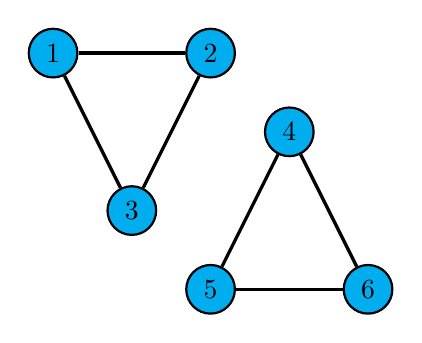
\begin{tikzpicture}
    \begin{scope}[every node/.style={circle,thick,draw,fill=cyan}]%text=white}]
      \node (1) at (0,2) {1};
      \node (2) at (2,2) {2};
      \node (3) at (1,0) {3};
      \node (4) at (3,1) {4};
      \node (5) at (2,-1) {5};
      \node (6) at (4,-1) {6};
    \end{scope}

    \begin{scope}[>={Stealth[black]},
        every node/.style={fill=white,circle},
        every edge/.style={draw=black,very thick}]
      \path (1) edge (2);
      \path (2) edge (3);
      \path (3) edge (1);
      \path (4) edge (5);
      \path (5) edge (6);
      \path (6) edge (4);
    \end{scope}
  \end{tikzpicture}
\end{columns}

\vspace{.5cm}

Verify that the two zero eigenvectors are $(1,1,1,0,0,0)$ and $(0,0,0,1,1,1)$ corresponding to the connected components.

\end{frame}

\begin{frame}
  \frametitle{The incidence matrix}

  For a directed graph (every edge has an orientation) $G=(V,E)$ with
$N$ nodes and $L$ edges, the node-edge \alert{incidence matrix}
$K\in\R^{N\times L}$ has components
\begin{align*}
K_{i\ell} = \begin{cases}
\phantom{-} 1 & \text{ if edge $\ell$ starts at node $i$} \\
-1 & \text{ if edge $\ell$ ends at node $i$} \\
\phantom{-} 0 & \text{ otherwise}
\end{cases}
\end{align*}
\begin{columns}
\column[c]{.5\textwidth}
\begin{equation*}
\mathbf{K}=\left(\begin{matrix}
1 & 0 & 0 & 0\\
-1 & 1 & 1 & 0\\
0 & -1 & 0 & 1\\
0 & 0 & -1 & -1
\end{matrix}\right)
\end{equation*}
    \column[c]{.5\textwidth}

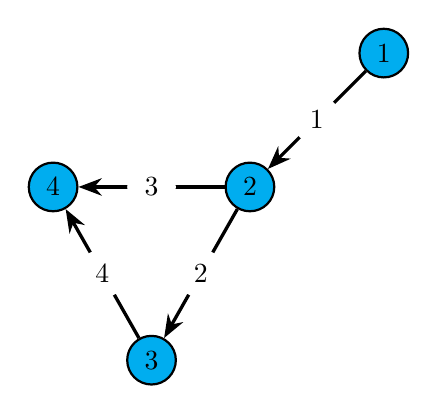
\begin{tikzpicture}
    \begin{scope}[every node/.style={circle,thick,draw,fill=cyan}]%text=white}]
      \node (4) at (0,2.5) {4};
      \node (2) at (2.5,2.5) {2};
      \node (3) at (1.25,.3) {3};
      \node (1) at (4.2,4.2) {1};
    \end{scope}

    \begin{scope}[>={Stealth[black]},
        every node/.style={fill=white,circle},
        every edge/.style={draw=black,very thick}]
      \path [->] (1) edge node {1} (2);
      \path [->] (2) edge node {2} (3);
      \path [->] (3) edge node {4} (4);
      \path [->] (2) edge node {3} (4);
    \end{scope}
  \end{tikzpicture}
\end{columns}
\end{frame}



\begin{frame}
  \frametitle{Incidence matrix properties}

  The incidence matrix has several important properties.

  First, for a given edge $\ell$, the corresponding column sums to zero $\sum_{i} K_{i\ell} = 0$, since every edge starts at some node (+1) and ends at some node (-1).

  The row corresponding to each node $i$ tells you which edges start there (+1) and which edges end there (-1).

  It is related to the Laplacian matrix by
  \begin{equation*}
    L = KK^t
  \end{equation*}

  Check the definitions agree:
  \begin{equation*}
    L_{ij} = \sum_\ell K_{i\ell}K_{j\ell}
  \end{equation*}
  for $i=j$ and $i\neq j$.

\end{frame}



\begin{frame}
  \frametitle{Incidence matrix properties}

  Let's verify:
  \begin{equation*}
    L_{ij} = \sum_\ell K_{i\ell}K_{j\ell}
  \end{equation*}

  For $i=j$ we get
  \begin{equation*}
    L_{ii} = \sum_\ell \left(K_{i\ell}\right)^2
  \end{equation*}
  The summands are only non-zero if the line $\ell$ is attached to $i$, so we get the degree
  \begin{equation*}
    L_{ii} = k_i
  \end{equation*}
  Correct!

  For $i\neq j$ we have
  \begin{equation*}
    L_{ij} = \sum_\ell K_{i\ell}K_{j\ell}
  \end{equation*}
  If there is no line between $i$ and $j$, then both sides are zero.

  If there is a line between $i$ and $j$ one of $K_{i\ell}$ and $K_{j\ell}$ is $+1$, while the other is $-1$, so we get $L_{ij} = -1$. Correct!


\end{frame}

\begin{frame}
  \frametitle{The kernel of the incidence matrix}

  The kernel of $K_{i\ell}$, i.e. particular combinations of edges which
  are annihilated by $K$, has a very special meaning.

  Consider the combination of edges $(0,1,-1,1)^t$

  \begin{equation*}
\mathbf{K}\left(\begin{matrix}
0 \\
1 \\
-1 \\
1
\end{matrix}\right)=\left(\begin{matrix}
1 & 0 & 0 & 0\\
-1 & 1 & 1 & 0\\
0 & -1 & 0 & 1\\
0 & 0 & -1 & -1
\end{matrix}\right)\left(\begin{matrix}
0 \\
1 \\
-1 \\
1
\end{matrix}\right) = \left(\begin{matrix}
0 \\
0 \\
0 \\
0
\end{matrix}\right)
\end{equation*}

  This corresponds to a \alert{cycle} in the graph. A cycle is a path
  through the network that returns to its starting node. Each node
  in the cycle has an edge that ends there and an edge that starts
  there, so is annihilated by $K$.

  The matrix $K$ can be interpreted as a \alert{boundary operator}. A
  cycle has no boundary in 0-d. There is a general theory called
  \alert{homology theory}, which can compute topological invariants of
  manifolds called \alert{homology groups}.

\end{frame}


\begin{frame}
  \frametitle{A cycle}

\begin{columns}
    \column[c]{.5\textwidth}

    For our graph:
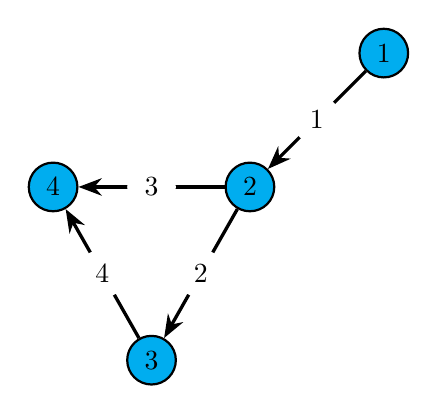
\begin{tikzpicture}
    \begin{scope}[every node/.style={circle,thick,draw,fill=cyan}]%text=white}]
      \node (4) at (0,2.5) {4};
      \node (2) at (2.5,2.5) {2};
      \node (3) at (1.25,.3) {3};
      \node (1) at (4.2,4.2) {1};
    \end{scope}

    \begin{scope}[>={Stealth[black]},
        every node/.style={fill=white,circle},
        every edge/.style={draw=black,very thick}]
      \path [->] (1) edge node {1} (2);
      \path [->] (2) edge node {2} (3);
      \path [->] (3) edge node {4} (4);
      \path [->] (2) edge node {3} (4);
    \end{scope}
  \end{tikzpicture}

\column[c]{.5\textwidth}
The combination  of edges $(0,1,-1,1)^t$ corresponds to the cycle:

\vspace{.5cm}

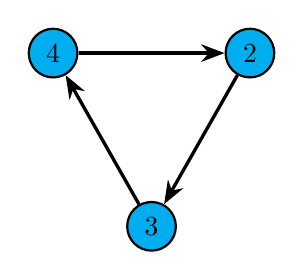
\begin{tikzpicture}
    \begin{scope}[every node/.style={circle,thick,draw,fill=cyan}]%text=white}]
      \node (4) at (0,2.5) {4};
      \node (2) at (2.5,2.5) {2};
      \node (3) at (1.25,.3) {3};
    \end{scope}

    \begin{scope}[>={Stealth[black]},
        every node/.style={fill=white,circle},
        every edge/.style={draw=black,very thick}]
      \path [->] (2) edge (3);
      \path [->] (3) edge (4);
      \path [->] (4) edge (2);
    \end{scope}
  \end{tikzpicture}

\vspace{.5cm}

NB: The direction of edge 3 is reversed by the minus sign.

\end{columns}

\end{frame}




\begin{frame}
  \frametitle{Cycle matrix}

  We can organise the cycles in a matrix $C_{\ell c}$, where $c$ labels each cycle.

  We have
  \begin{equation*}
    KC = 0
  \end{equation*}
  by definition of $C$ being in the kernel.

  The image of $K$ has dimension $N-1$ (i.e. the rank of $K$) for a connected graph, since
  the space spanned by the columns of $K$ can only reach differences
  between nodes and never then $N$-length vector $(1,1,\dots 1)^t$.

  By the rank-nullity theorem for $K$ we have
  \begin{equation*}
    L = \textrm{dim}\,\textrm{im} K + \textrm{dim}\,\textrm{ker} K
  \end{equation*}
  so the number of cycles, i.e. the dimension of the kernel (nullity) of $K$ is $L-N+1$.
  If the connected graph has no cycles, i.e. it is a tree, then $L = N-1$.

  In our case $L = 4$, $N = 4$ so there is only 1 cycle
  \begin{equation*}
    \mathbf{C} = (0,1,-1,1)^t
  \end{equation*}

\end{frame}
%-----%-----%-----%-----%-----%-----%-----%-----%



\begin{frame}
  \frametitle{Independent basis of cycles}

  \begin{circuitikz}
  \draw
  (0,3)
  to [short,i^=$f_1$,*-*] (3,3)
  to [short,i>=$f_2$,*-*] (3,0)
  to [short,i>=$f_3$,*-*] (0,0)
  to [short,i>=$f_4$,*-*] (0,3);
  \draw (3,3)   to [short,i^=$f_5$,*-*] (0,0);

  \draw[blue]
  (5,3)
  to [short,i>=$$,*-*] (7.8,3)
  to [short,i>=$$,*-*] (5,0.2)
  to [short,i>=$c_1$,*-*] (5,3);

  \draw[blue]
  (8,0)
  to [short,i>=$$,*-*] (5.2,0)
  to [short,i>=$$,*-*] (8,2.8)
  to [short,i>=$c_2$,*-*] (8,0);


\end{circuitikz}

  Two independent cycles:

  $c_1 = f_1 + f_5 + f_4$

  $c_2 = f_2 + f_3 + -f_5$

  The outer cycle is not independent:

  $c_3  = f_1 + f_2 + f_3 + f_4 = c_1 + c_2$

\end{frame}







\begin{frame}
\frametitle{Trees}
\begin{columns}
\column[c]{.5\textwidth}
\begin{itemize}
\item Trees play an import role for random graph models.
\item In a tree, there is exactly one path between any pair of vertices.
\item A tree of $N$ vertices always has exactly $N-1$ edges.
\item Any connected network with~$N$ vertices and $N-1$ edges is a tree.
  \item Trees have \alert{no cycles}.
\item A collection of trees is called a \alert{forest}.
\end{itemize}
    \column[c]{.5\textwidth}
\includegraphics[scale=0.12]{graph22.png}
\end{columns}
\end{frame}
%-----%-----%-----%-----%-----%-----%-----%-----%
\begin{frame}
\frametitle{Planar networks}
A \alert{planar network} is a network that can be drawn on a plane without having any edges cross.\\
\vspace{0.5cm}
\begin{columns}
\column[c]{.5\textwidth}
Examples:
\begin{itemize}
\item Trees
\item Road networks (approximately)
\item Power grids (approximately)
\item Shared borders between countries, etc.
\end{itemize}
    \column[c]{.5\textwidth}
\includegraphics[scale=0.12]{graph23.png}
\end{columns}
\end{frame}
%-----%-----%-----%-----%-----%-----%-----%-----%
\begin{frame}
\frametitle{Paths}
\begin{itemize}
\item Route through the network, from vertex to vertex along the edges
\item Defined for both directed and undirected networks
\item Special case: self-avoiding paths
\item \alert{Length} of a path: number of edges along the path ("hops")
\item Number of paths of length $r$ between vertices $i$ and $j$:
\begin{equation*}
N_{ij}^{(r)}=\left[\mathbf{A}^{r}\right]_{ij}
\end{equation*}
\item Total number $L_{r}$ of loops of length $r$ anywhere in the network:
\begin{equation*}
L_{r}=\sum_{i=1}^{n}\left[\mathbf{A}^{r}\right]_{ii}=\text{Tr}\mathbf{A}^{r}~.
\end{equation*}
\end{itemize}
\end{frame}
%-----%-----%-----%-----%-----%-----%-----%-----%
\begin{frame}
\frametitle{Geodesic / shortest paths}
\begin{columns}
\column[c]{.6\textwidth}
\begin{itemize}
\item A path between two vertices such that no shorter path exists
\item Geodesic distance between vertices $i$ and $j$ is the smallest value of $r$ such that
$\left[\mathbf{A}^{r}\right]_{ij}>0$.
\item Self-avoiding
\item In general not unique
\item \alert{Diameter} of a network: Length of the longest geodesic path between any pair of vertices
\end{itemize}
\column[c]{.4\textwidth}
\includegraphics[scale=0.12]{graph26.png}
\end{columns}
\end{frame}

%-----%-----%-----%-----%-----%-----%-----%-----%
\begin{frame}
\frametitle{Acyclic directed network}
\begin{columns}
\column[c]{.6\textwidth}
\begin{itemize}
\item Directed network without cycles of edges (DAG)
\item Examples: power flow in an electricity grid, citation network of papers
\item Topological ordering: For every directed edge $i\to j$, vertex $i$ comes before $j$ in the ordering:\\(1,2,3,4,6,9,10,11,12,8,7,5,13)
\item With a topological ordering, the adjacency matrix of an acyclic directed network is \alert{strictly triangular}
\end{itemize}
\column[c]{.4\textwidth}
\includegraphics[scale=0.12]{graph13.png}
\end{columns}
\end{frame}



\begin{frame}
\frametitle{Why is it called the Laplacian?}

What does this matrix have to do with the second-order Laplacian:
\begin{equation}
  \Delta = \frac{\partial^2}{\partial x^2} + \frac{\partial^2}{\partial y^2} + \frac{\partial^2}{\partial z^2}
\end{equation}
from continuous physics?

On a 1d lattice, for each link (difference) from $K^t$ get $u_i - u_{i-1} \sim \frac{d}{dx}$.
 From $L = KK^t$ get $2u_i - u_{i-1} - u_{i+1} \sim \frac{d^2}{dx^2}$.

Similarly for 2d lattice, from the Laplacian you get
\begin{equation}
  4u_{i,j} - u_{i+1,j} - u_{i-1,j} - u_{i,j+1} - u_{i,j-1}  \sim \frac{\partial^2}{\partial x^2} + \frac{\partial^2}{\partial y^2}
\end{equation}
which is a second-order difference in both $x$ and $y$ directions.

In fact you can do interesting discrete physics with these matrices
(more later...).



\end{frame}



\begin{frame}
  \frametitle{(Co)homology analogy}


  \begin{align*}
    K  & \leftrightarrow  \delta \textrm{ (1d boundary operator)} \\
    K^t  & \leftrightarrow  d \textrm{ (0d differential)} \\
   L = KK^t & \leftrightarrow \Delta = d*d \textrm{ (0d Laplacian)}
  \end{align*}


  On a 1d lattice, for each link (difference) from $K^t$ get $u_i - u_{i-1} \sim \frac{d}{dx}$.
  From $L = KK^t$ get $2u_i - u_{i-1} - u_{i+1} \sim \frac{d^2}{dx^2}$.

  Similarly for 2d lattice.
\end{frame}




\section{Computing the Linear Power Flow}




\begin{frame}
  \frametitle{The goal of power flow analysis}

  \begin{columns}
    \column[c]{.55\textwidth}

  The goal of a power/load flow analysis is to find the flows in the
  lines of a network given a power injection pattern at the nodes.


    I.e. given power injection at the nodes
\begin{equation*}
\mathbf{P}_{i}=\left(\begin{matrix}
50 \\
50 \\
0 \\
-100
\end{matrix}\right)
\end{equation*}
what are the flows in lines 1-4?

\vspace{.1cm}

To find the flows, it is sufficient to know the \alert{impedances} of
the lines and the \alert{voltages} at each node.

\column[c]{.45\textwidth}
\includegraphics[scale=0.12]{graph19.png}
\end{columns}


\end{frame}



\begin{frame}
  \frametitle{Framing the load flow problem}

  Suppose we have $N$ nodes labelled by $i$, and $L$ edges labelled by
  $\ell$ forming a directed graph $G$.

  Suppose at each node we have a \alert{power imbalance} $p_i$ ($p_i >
  0$ means its generating more than it consumes and $p_i < 0$ means it
  is consuming more than it).

  Since we cannot create or destroy energy (and we're ignoring losses):
  \begin{equation*}
    \sum_i p_i = 0
  \end{equation*}

  \alert{Question}: How do the flows $f_\ell$ in the network relate to the nodal power
  imbalances?

  \alert{Answer}: According to the impedances (generalisation of
  resistance for oscillating voltage/current) and the corresponding
  voltages.

\end{frame}



\begin{frame}
  \frametitle{Ohm's Law}

  \alert{Ohm's Law}: The potential difference (voltage) $V_1 - V_2$ across an ideal conductor is proportional to the current through it $I$. The constant of proportionality is called the \alert{resistance}, $R$. Ohm's Law is thus:
  \begin{equation*}
     V_1 - V_2 = I\,R
  \end{equation*}

  \centering
  \includegraphics[width=8cm]{ohm_law.png}


\end{frame}

\begin{frame}
  \frametitle{Analogy DC circuits to linear power flow}

  The equations for DC circuits and linear power flow in AC circuits are analogous:
  \begin{equation*}
    I = \frac{V_i - V_j}{R} \hspace{.55cm} \leftrightarrow \hspace{.55cm} f_\ell =  \frac{\theta_i - \theta_j}{x_\ell}
  \end{equation*}

  if we make the following identification:
    \ra{1.05}
  \begin{table}[!t]
    \begin{tabular}{p{4cm}p{0.5cm}p{4cm}}
      \toprule
      Current flow $I$ & $\leftrightarrow$  &  Active power flow $f_\ell$ \\
      Potential/voltage $V_i$ & $\leftrightarrow$  &  Voltage angle $\theta_i$ \\
      Resistance $R$ & $\leftrightarrow$  &  Reactance $X$ \\
      \bottomrule
    \end{tabular}
  \end{table}

  The simplifications that lead to the linear power flow will be explained in the next lecture.

\end{frame}


\begin{frame}
  \frametitle{Kirchhoff's Current Law (KCL)}

  KCL inforces energy conservation at each vertex (the power imbalance
  equals what goes out minus what comes in).

  \vspace{.3cm}

  \begin{columns}
    \column[c]{.5\textwidth}


    \centering

  %https://tex.stackexchange.com/questions/270543/draw-a-graph-in-latex-with-tikz
  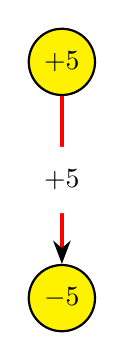
\begin{tikzpicture}
    \begin{scope}[every node/.style={circle,thick,draw,fill=yellow}]
      \node (1) at (0,3) {$+5$};
      \node (2) at (0,0) {$-5$};
    \end{scope}

    \begin{scope}[>={Stealth[black]},
        every node/.style={fill=white,circle},
        every edge/.style={draw=red,very thick}]
      \path [->] (1) edge node {$+5$} (2);
    \end{scope}
  \end{tikzpicture}

    \column[c]{.5\textwidth}


    \centering

  %https://tex.stackexchange.com/questions/270543/draw-a-graph-in-latex-with-tikz
  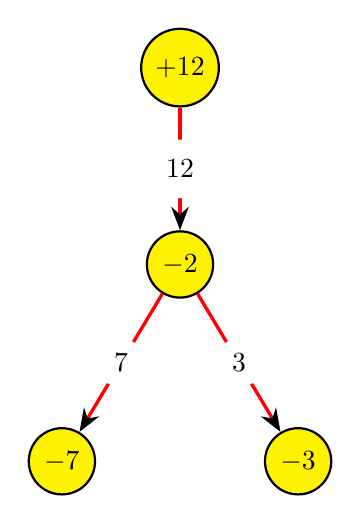
\begin{tikzpicture}
    \begin{scope}[every node/.style={circle,thick,draw,fill=yellow}]
      \node (1) at (1.5,5) {$+12$};
      \node (2) at (1.5,2.5) {$-2$};
      \node (3) at (0,0) {$-7$};
      \node (4) at (3,0) {$-3$};
    \end{scope}

    \begin{scope}[>={Stealth[black]},
        every node/.style={fill=white,circle},
        every edge/.style={draw=red,very thick}]
      \path [->] (1) edge node {$12$} (2);
      \path [->] (2) edge node {$7$} (3);
      \path [->] (2) edge node {$3$} (4);
    \end{scope}
  \end{tikzpicture}


  \end{columns}

\end{frame}



\begin{frame}
  \frametitle{Kirchhoff's Current Law (KCL)}

  KCL says (in this linear setting) that the nodal power imbalance at
  node $i$ is equal to the sum of direct flows arriving at the
  node. This can be expressed compactly with the incidence matrix

  \begin{equation*}
    p_i = \sum_\ell K_{i\ell} f_\ell \hspace{2cm} \forall i
  \end{equation*}


\end{frame}



\begin{frame}
  \frametitle{Kirchhoff's Voltage Law (KVL)}

  KCL isn't enough to determine the flow as soon as there are \alert{closed cycles} in the network.
   For this we need Ohm's law in combination with KVL: voltage
  differences around each cycle add up to zero.

  \vspace{.3cm}

  \begin{columns}
    \column[c]{.5\textwidth}


    \centering

  %https://tex.stackexchange.com/questions/270543/draw-a-graph-in-latex-with-tikz
  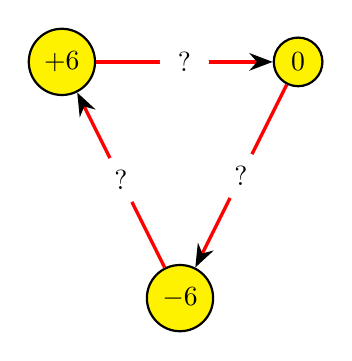
\begin{tikzpicture}
    \begin{scope}[every node/.style={circle,thick,draw,fill=yellow}]
      \node (1) at (0,3) {$+6$};
      \node (2) at (3,3) {$0$};
      \node (3) at (1.5,0) {$-6$};
    \end{scope}

    \begin{scope}[>={Stealth[black]},
        every node/.style={fill=white,circle},
        every edge/.style={draw=red,very thick}]
      \path [->] (1) edge node {$?$} (2);
      \path [->] (2) edge node {$?$} (3);
      \path [->] (3) edge node {$?$} (1);
    \end{scope}
  \end{tikzpicture}


      \column[c]{.5\textwidth}


      For equal reactances for each edge:


  \vspace{.3cm}

    \centering
  %https://tex.stackexchange.com/questions/270543/draw-a-graph-in-latex-with-tikz
  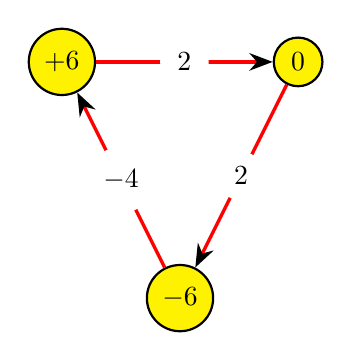
\begin{tikzpicture}
    \begin{scope}[every node/.style={circle,thick,draw,fill=yellow}]
      \node (1) at (0,3) {$+6$};
      \node (2) at (3,3) {$0$};
      \node (3) at (1.5,0) {$-6$};
    \end{scope}

    \begin{scope}[>={Stealth[black]},
        every node/.style={fill=white,circle},
        every edge/.style={draw=red,very thick}]
      \path [->] (1) edge node {$2$} (2);
      \path [->] (2) edge node {$2$} (3);
      \path [->] (3) edge node {$-4$} (1);
    \end{scope}
  \end{tikzpicture}

  \raggedright
  NB: For directed graph, sign determines direction of flow.

  \end{columns}
\end{frame}



\begin{frame}
  \frametitle{Kirchhoff's Voltage Law (KVL)}

  KVL says that the sum of voltage differences across edges for any
  closed cycle must add up to zero.

  If the voltage at any node is given by $\theta_i$ (this is infact
  the voltage \alert{angle} - more next time) then the voltage difference across edge $\ell$ is
  \begin{equation*}
    \sum_i K_{i\ell} \theta_i
  \end{equation*}

  And Kirchhoff's law can be expressed using the cycle matrix encoding of independent cycles
  \begin{equation*}
    \sum_\ell C_{\ell c} \sum_i K_{i\ell} \theta_i = 0 \hspace{2cm} \forall c
  \end{equation*}

  [Automatic, since we already said KC = 0.]


\end{frame}



\begin{frame}
  \frametitle{Kirchhoff's Voltage Law (KVL)}

  If we express the flow on each line in terms of the voltage angle (a
  relative of $V = IR$) then for a line $\ell$ with reactance $x_\ell$
  \begin{equation*}
    f_\ell = \frac{\theta_i - \theta_j}{x_\ell} = \frac{1}{x_\ell}\sum_{i} K_{i\ell} \theta_i
  \end{equation*}

  KVL now becomes
  \begin{equation*}
    \sum_\ell C_{\ell c} x_\ell f_\ell = 0 \hspace{2cm} \forall c
  \end{equation*}

\end{frame}



\begin{frame}
  \frametitle{Solving the equations}

  If we combine
    \begin{equation*}
    f_\ell  = \frac{1}{x_\ell}\sum_{i} K_{i\ell} \theta_i
  \end{equation*}
    with Kirchhoff's Current Law we get
    \begin{equation*}
    p_i = \sum_{\ell} K_{i\ell}f_\ell =   \sum_{\ell} K_{i\ell} \frac{1}{x_\ell}\sum_{j} K_{j\ell} \theta_j
    \end{equation*}
    This is a \alert{weighted Laplacian}. If we write $B_{k\ell}$ for the diagonal matrix with $B_{\ell\ell} = \frac{1}{x_\ell}$ then
    \begin{equation*}
      L = KBK^t
    \end{equation*}
    and we get a \alert{discrete Poisson equation} for the $\theta_i$ sourced by the $p_i$
    \begin{equation*}
      p_i = \sum_{j} L_{ij} \theta_j
    \end{equation*}
    We can solve this for the $\theta_i$ and thus find the flows.

\end{frame}



\begin{frame}
  \frametitle{Solving the equations}

  Given $p_i$ at every node, we want to find the flows $f_\ell$. We
  have the equations
    \begin{align*}
      p_i & = \sum_{j} L_{ij} \theta_j \\
     f_\ell  & = \frac{1}{x_\ell}\sum_{i} K_{i\ell} \theta_i
    \end{align*}

    Basic idea: invert $L$ to get $\theta_i$ in terms of $p_i$
    \begin{equation*}
      \theta_i  = \sum_{k} (L^{-1})_{ik} p_k
    \end{equation*}
    then insert to get the flows as a linear function of the power injections $p_i$
    \begin{equation*}
    f_\ell   = \frac{1}{x_\ell}\sum_{i,k} K_{i\ell}  (L^{-1})_{ik} p_k = \sum_k \textrm{PTDF}_{\ell k} p_k
    \end{equation*}
    called the \alert{Power Transfer Distribution Factors} (PTDF).

    The catch: $L$ is not invertible because of the zero eigenvalues. More next time!
\end{frame}

\end{document}
